\section{Opis Operatora}

\subsection{Plus - Polkomtel Sp. z o.o.}

\begin{flushleft}

    Polkomtel Sp. z o.o. to operator telekomunikacyjny w Polsce, świadczący usługi pod marką Plus. Jest częścią Grupy Polsat Plus, grupy medialno-telekomunikacyjnej w Polsce dostarczającej swoim klientom łącznie ponad 20 mln usług telefonii komórkowej, płatnej telewizji i dostępu do Internetu.

    \begin{figure}[!htb]
        \centering
        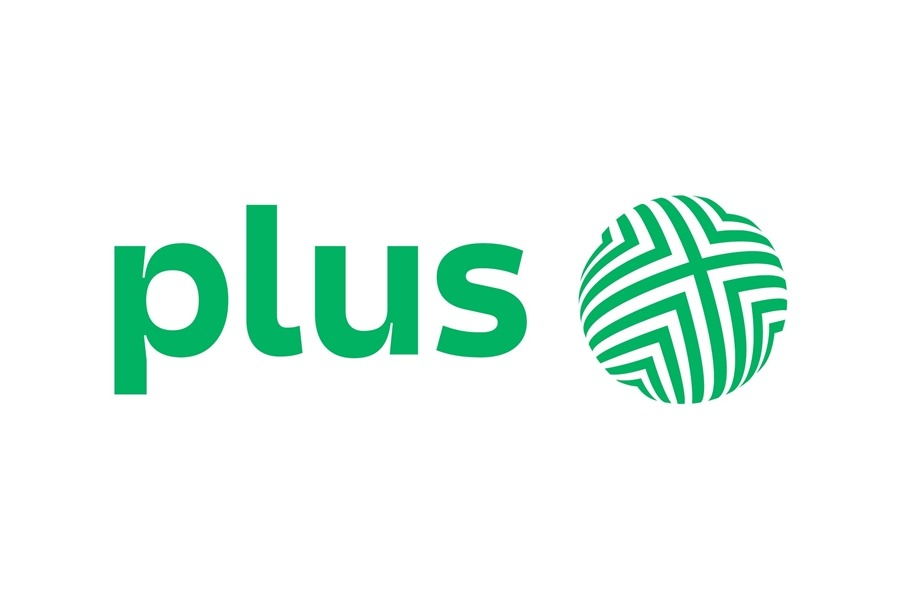
\includegraphics[width=0.4\textwidth]{plus-logo}
        \caption{Aktualne logo sieci od 2021 r.}
    \end{figure}

    \begin{figure}[!htb]
        \centering
        
\includegraphics[width=0.4\textwidth]{stare-logo}
        \caption{Logotyp firmy stosowany od 1996 r.}
    \end{figure}
        
\end{flushleft}


\subsection{Zasięg Operatora}
    \begin{flushleft}
        Jego zasięg obejmuje zarówno obszary miejskie, jak i wiejskie, co sprawia, że jest to operator o zasięgu ogólnopolskim. Obecnie już 20 mln mieszkańców Polski może korzystać z 5G w Plusie.

        \begin{figure}[!htb]
            \centering
            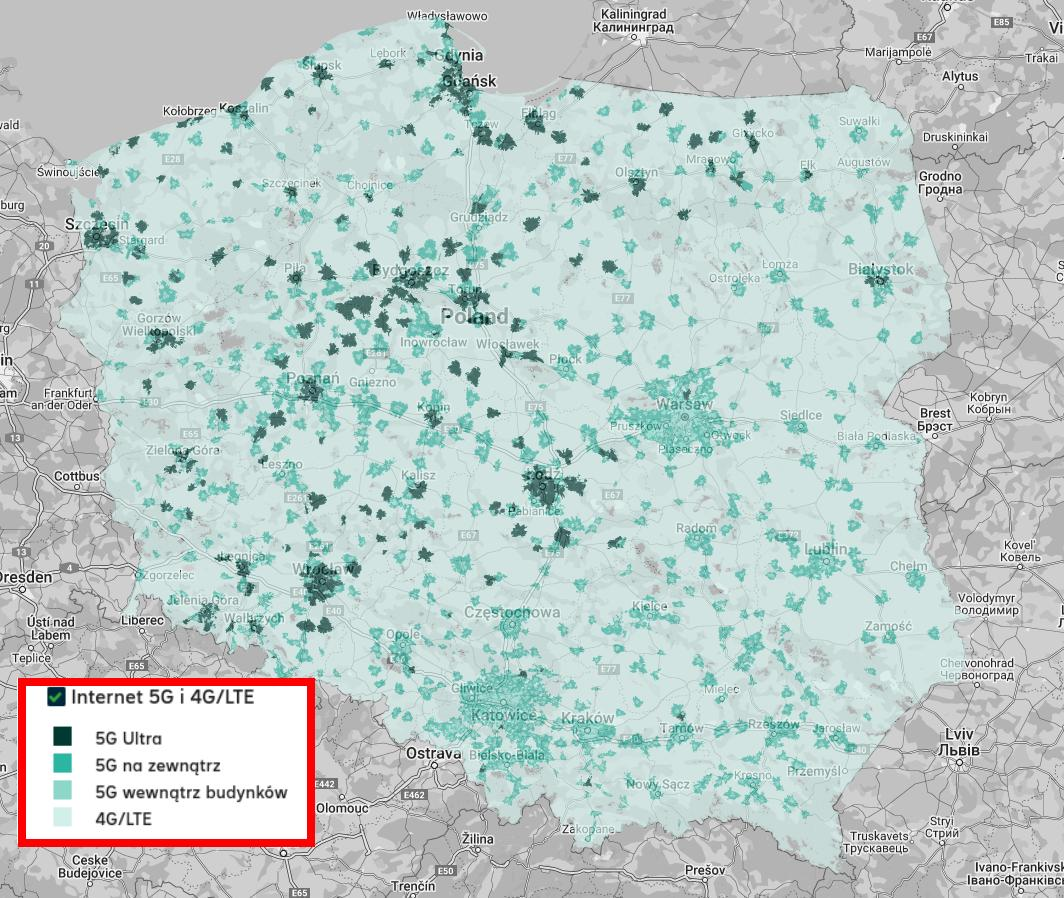
\includegraphics[width=0.8\textwidth]{mapa-5g}
            \caption{Aktualny zasięg sieci 5G oraz 4G LTE Plus w Polsce}
        \end{figure}
    
        \begin{figure}[!htb]
            \centering
            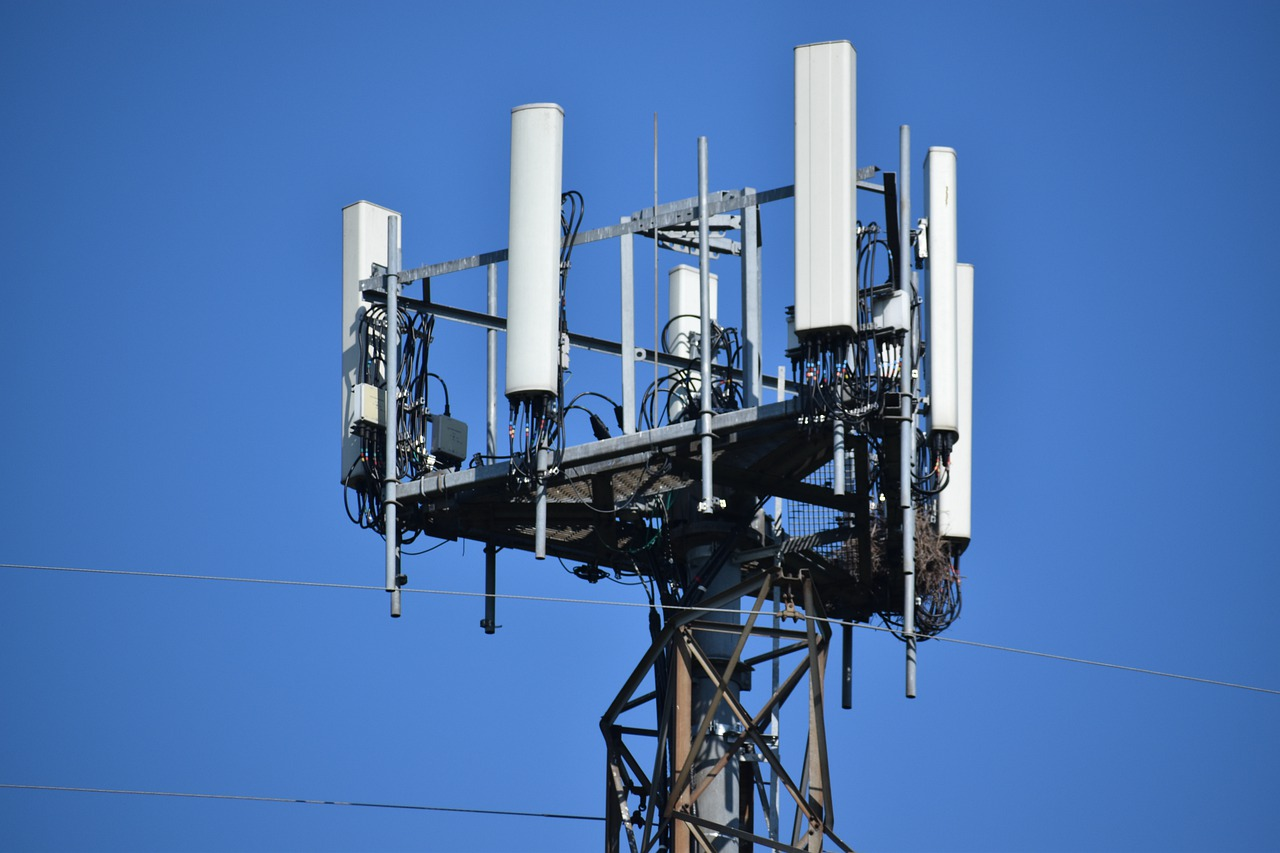
\includegraphics[width=0.4\textwidth]{maszt}
            \caption{Maszt 5G operatora Plus}
        \end{figure}

    \end{flushleft}
    
    \pagebreak

\subsection{Dostępne Technologie Podłączeń}
Plus oferuje szereg różnych technologii podłączeń internetu mobilnego, w tym:
\begin{itemize}
    \item 3G (HSPA, HSPA+)
    \item 4G LTE (Long Term Evolution)
    \item 5G (piąta generacja technologii komórkowych)
\end{itemize}

\subsection{Oferowane Technologie Połączenia}
Klienci operatora Plus mogą korzystać z następujących technologii połączenia:
\begin{itemize}
    \item Połączenie GSM (Global System for Mobile Communications)
    \item Połączenie LTE (Long Term Evolution)
    \item Połączenie 5G NR (5G New Radio)
\end{itemize}

\subsection{Pasma Transmisyjne}
Plus oferuje różne pasma transmisyjne, w tym:
\begin{itemize}
    \item Dla technologii 3G: pasmo 2100 MHz
    \item Dla technologii LTE: pasmo 800 MHz, 1800 MHz, 2600 MHz
    \item Dla technologii 5G: pasma n78 (3500 MHz), n41 (2500 MHz)
\end{itemize}

\subsection{Oferta Cenowa}

Oferta cenowa operatora Plus jest zróżnicowana i obejmuje różne pakiety danych oraz usługi dodatkowe. Ceny zależą od wybranej technologii, prędkości internetu i ilości danych w pakiecie. Oferta dla klientów indywidualnych różni się od oferty skierowanej dla firm.

\begin{figure}[!htb]
    \centering
    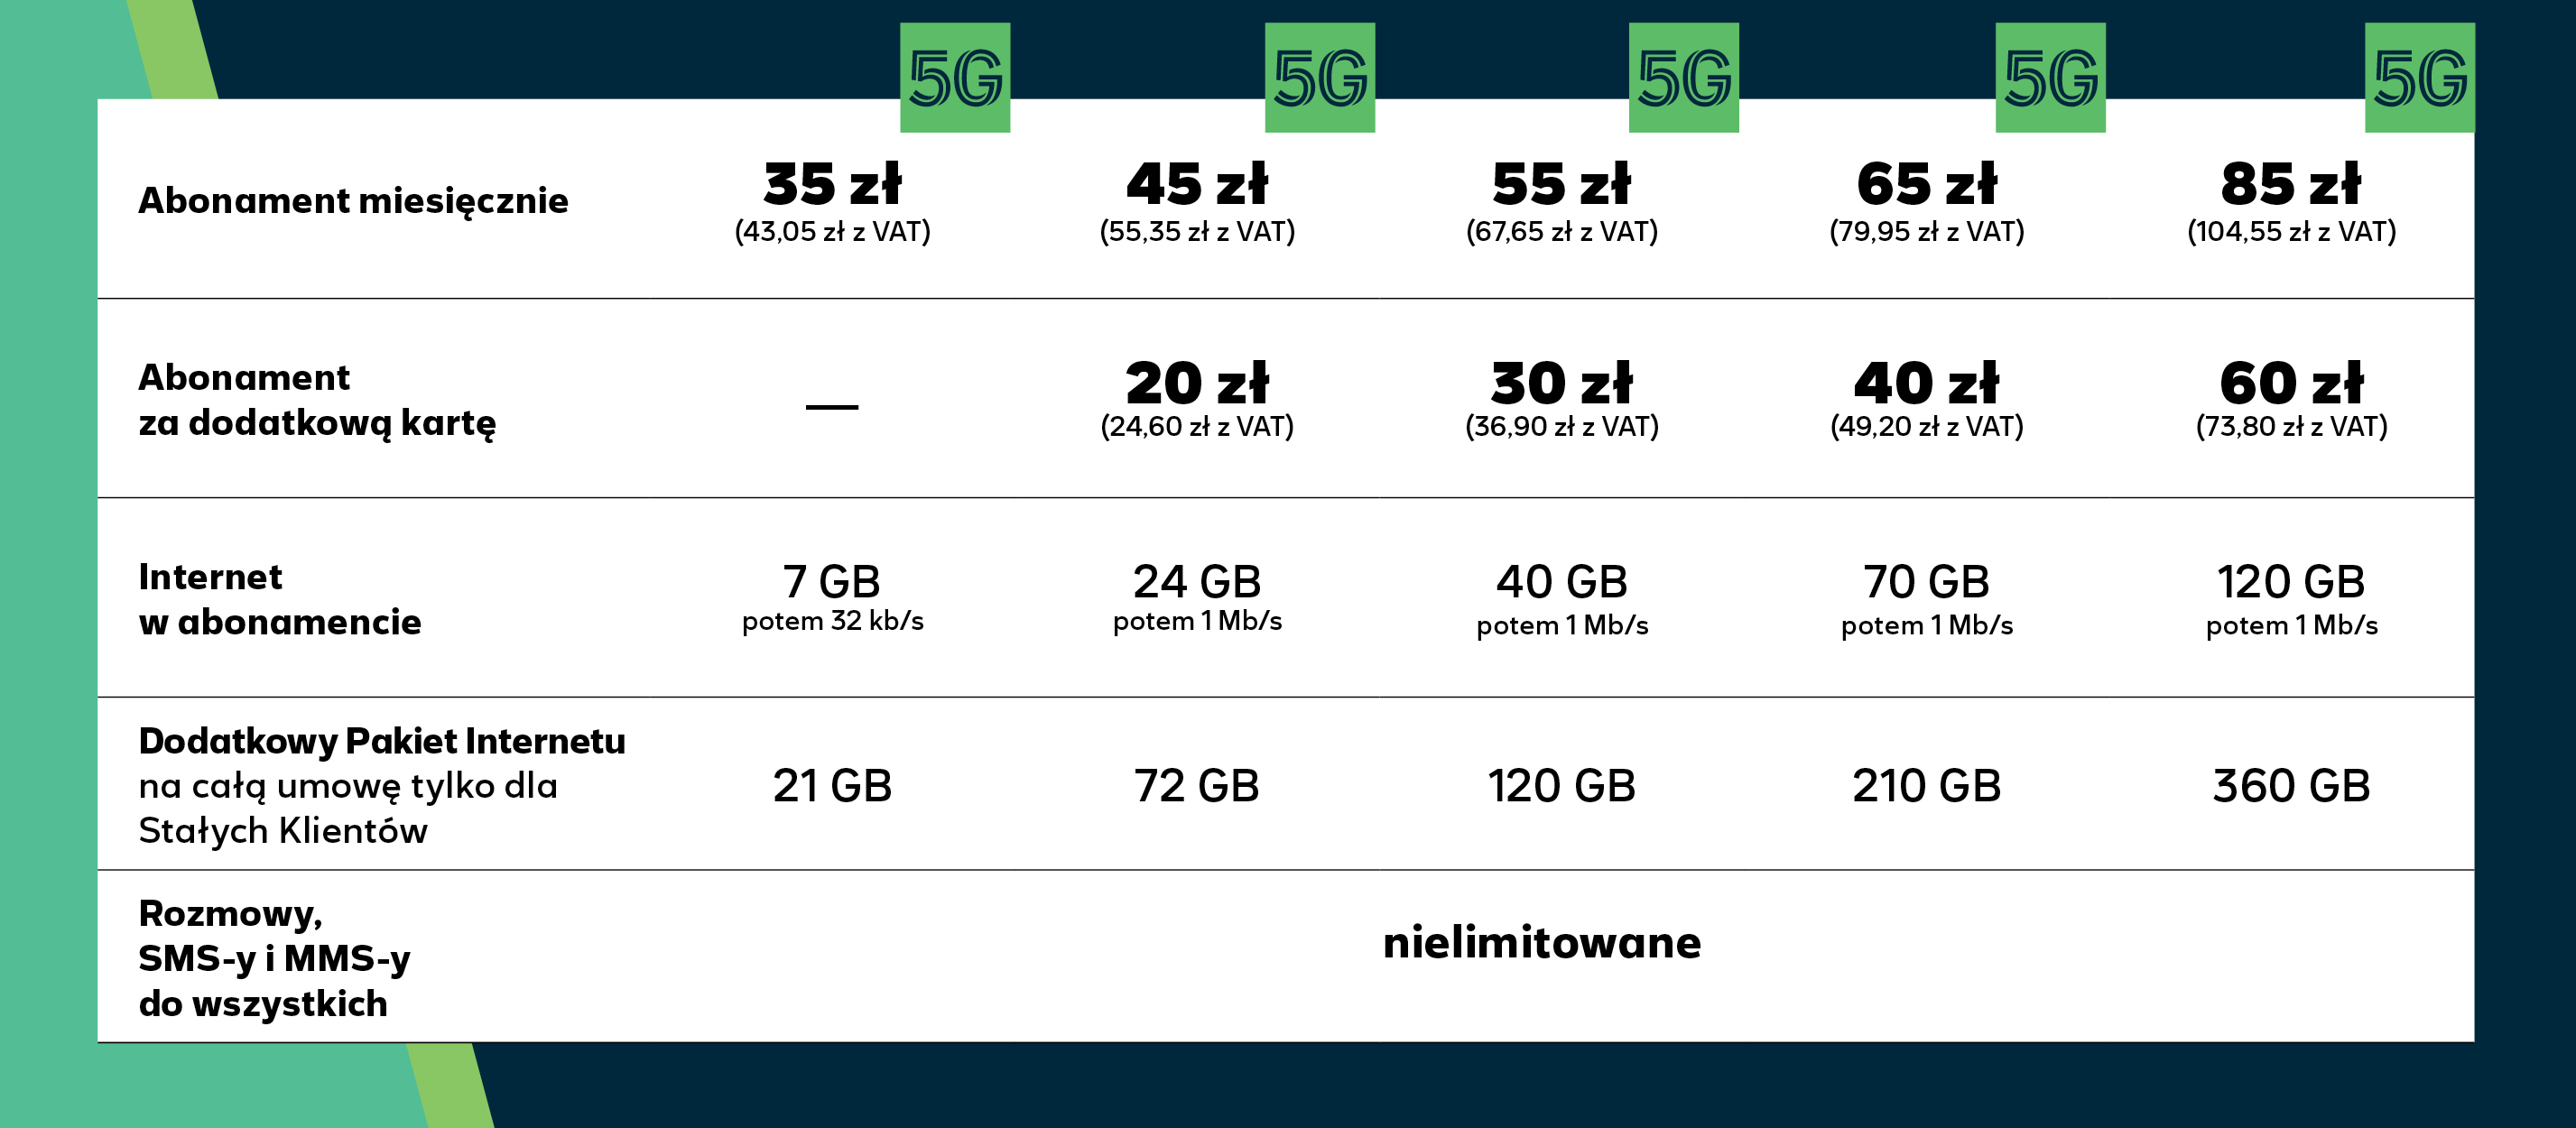
\includegraphics[width=0.6\textwidth]{oferta}
    \caption{Przykładowa oferta dla internetu 5G}
\end{figure}


